%!TEX root=seke.tex
% mainfile: seke.tex

\documentclass[10pt,twocolumn]{article}

\usepackage[table]{xcolor}% http://ctan.org/pkg/xcolor
\usepackage{latex8}
\usepackage{times}
\usepackage{pifont}

% \usepackage[numbers]{natbib}
\usepackage{graphicx}
\usepackage{algorithm}
\usepackage{algorithmic}

\usepackage{tikz}
\usetikzlibrary{shapes,arrows,shadows}
\usepackage{amsmath,bm,times}
\usepackage{verbatim}

\newcommand{\goallegheny}{$^{\mbox{\footnotesize \ding{72}}}$}
\newcommand{\gosheffield}{$^{\mbox{\footnotesize \ding{73}}}$}
\newcommand{\gospace}{$\;$}

\begin{document}

% \title{Empirically Evaluating the Efficiency of Search-based \\ Test Data
% Generation for Relational Database Schemas\vspace*{-.1in}}

\title{Automatically Evaluating the Efficiency of Search-based \\ Test Data
Generation for Relational Database Schemas\vspace*{-.1in}}

\author{Cody Kinneer \goallegheny                \and
        Gregory M.\ Kapfhammer \goallegheny      \and
        Chris Wright \gosheffield                \and
        Phil McMinn \gosheffield \vspace*{-.1in}
      }

\affiliation{
      \goallegheny \gospace Allegheny College       \and
      \gosheffield \gospace University of Sheffield
}

\maketitle

\begin{abstract}

% When evaluating an algorithm, it is often useful to speak of it's efficiency in terms of it's worst-case complexity.
% This is the case for search-based test data generation tools.
% on the search-based data generation tool \textit{SchemaAnalyst}.

% This paper introduces a framework for conducting automated empirical studies of algorithms by doubling
% the size of the input and observing the change in runtime.

% After describing a way to systematically doubling the size of structured data, we report on a study demonstrating the
% presented method's effectiveness.

The characterization of an algorithm's worst-case time complexity is useful because it succinctly captures how algorithm
runtime will grow as the input size becomes arbitrarily large.  However, for certain algorithms---such as those
performing search-based test data generation---a theoretical analysis to determine worst-case complexity is cumbersome
and thus not reported in the literature.  This paper introduces a framework that empirically determines an algorithm's
worst-case time complexity by doubling the size of the input and observing the change in runtime.  Since the relational
database is a centerpiece of modern software and the database's schema is frequently untested, we apply the doubling
technique to the domain of data generation for relational database schemas, a field where worst-case time complexities
are unknown.  In addition to demonstrating the feasibility of suggesting the worst-case runtimes of the chosen
algorithms and configurations, the results of our study reveal performance trade-offs in schema testing strategies.

\end{abstract}

%!TEX root=../seke.tex
% mainfile: ../seke.tex

\vspace*{-.25in}
\section{Introduction}
\vspace*{-.05in}

% GMK NOTE: Removing the reference to the Walcott paper, not absolutely critical.

% Search-based algorithms allow the application of guidance to problems.
% The algorithm attempts to improve a potential
% solution until it is acceptable according to a fitness function.

Many disciplines, such as science, finance, and medicine, rely on relational databases to maintain large amounts of
critical information~\cite{kapfhammer2007}. The relational database schema defines the structure of a database and
protects the integrity of the data. This makes testing the database schema necessary to avoid the corruption of data.
Search-based algorithms, that use a fitness function to offer guidance to the correct solution, have been applied to
this challenging problem~\cite{kapfhammer2013}. Although data generation for relational schemas may also be solved,
albeit less effectively, with random generation techniques~\cite{mcminn2015}, the use of search-based approaches ensures
that data creation methods can actively seek out test inputs that best fulfill testing goals~\cite{mcminn2004a}.

% GMK NOTE: Revised this content in the paragraph above and below

% Without the use of a search-based strategy, a problem might be approached with a random sampling or greedy technique.
% In the domain of data generation for software testing, this means that rather than randomly selecting inputs from a
% program’s input space, the data generator can actively seek out qualities of an input that best fulfills the test’s
% goals~\cite{McMinn2004a}.

Despite the effectiveness of search-based data generation methods, there is, to the best of our knowledge, little prior
research that fully studies their efficiency and characterizes their worst-case time complexity. In part, we attribute
this dearth of past work to the fact that these systems are complex, thus making a generalizable theoretical analysis
hard.

In response to this lack of insight into the performance of search-based methods, this paper presents a fully automated
performance evaluation framework that employs doubling experiments to suggest worst-case time complexities and
classification and regression trees to identify efficiency trends. Applying this framework to the automated performance
evaluation of search-based test data generation for database schemas, the results reveal trade-offs in efficiency with
respect to the chosen testing goals, the structure of the relational schema, and the data generation strategy.

Since the presented approach is fully automated, it enabled a comprehensive study suggesting the worst-case time
complexity of all the relevant data generator configurations. Although this paper focuses on automatically evaluating
efficiency of search-based test data generation for database schemas, the presented technique is general and thus
applicable to a wide range of methods using heuristic search. In summary, this paper's important \mbox{contributions
include}:

% GMK NOTE: I captured the essence of this content and then made room for another key point

% attack the performance evaluation of search-based test data generation with an empirical
% approach. We present an empirical performance study of the search-based test data generation tool, called
% \textit{SchemaAnalyst}, which generates test suites for relational database schemas. To evaluate worst-case performance,
% we developed a technique for automatically conducting doubling experiments. Using this process, we explored
% \textsc{xmany} configurations of \textit{SchemaAnalyst}, revealing
% Our automatic technique enabled a comprehensive empirical study, that would otherwise have been infeasible, and the
% results have important practical significance for the selection of parameters in search-based test data generation
% tools.

\begin{enumerate}
  \itemsep0in

  \item A performance evaluation framework that automatically conducts and analyzes the results from doubling
    experiments with search-based methods.

  \item With a systematic focus on a wide variety of configurations, an empirical study revealing trade-offs
    in search-based test data generation for relational schemas.

  \item Empirically derived suggestions for the worst-case time complexity of search-based test data generators.

  \end{enumerate}
  \vspace*{-.15in}

%!TEX root=seke.tex
% mainfile: ../seke.tex

\section{Background and Related Work}

% Do we need to talk about databases/schemas/constraints?
% if so it should go here, and we're going to have major space issues

%TODO GMK: discuss database related content
%TODO GMK: Discuss coverage criterion
%TODO GMK: Explain the subsumption hierarchy
%TODO GMK: Discuss data generators

% \subsection{Search-Based Test Data Generation}

{\bf Testing Database Schemas.} The relational database, a cornerstone of modern software, is protected by a schema that
defines integrity constraints ensuring the coherence of data. These constraints defend the schema from manipulations
that could violate requirements such as ``user names must be unique'' or ``the host name cannot be missing or unknown''.
Prior work in this area proposed coverage criteria, derived from logic coverage criteria, that establish different
levels of testing for the formulation of integrity constraints in a database schema~\cite{mcminn2015}. These range from
simple criteria that mandate the testing of successful and unsuccessful INSERT statements into tables to more advanced
criteria that test the formulation of complex integrity constraints such as multi-column PRIMARY KEYs and arbitrary
CHECK constraints. This family of criteria has been organized into a subsumption hierarchy, with criterion such as {\em
Clause-Based Active Integrity Constraint Coverage} (ClauseAICC) emerging as a stringent testing strategy. Since space
constraints limit further commentary on testing methods for database schemas, the reader is referred
to~\cite{mcminn2015} for more details.

% Since the quality of the test depends upon the characteristics of the data itself, test data generators systematically
% produce test inputs according to a criterion. 

{\bf Search-Based Test Data Generation}. When testing a schema's integrity constraints for correctness, it is often
necessary to provide input to the database and observe and evaluate its execution~\cite{kapfhammer2013}.  Since the
database's behavior is dependant on the input from INSERTs, the input space must be sufficiently explored to ensure
thorough testing.  Due to the fact that it is challenging to manually create input that supports high-quality testing,
test data generation is used to automatically produce it according to a criterion, like ClauseAICC. A search-based test
data generator is one that explores that input space using, among other components, a fitness function that rates the
data's quality, thus allowing it to improve by repeatedly searching for better inputs~\cite{mcminn2004a}.

{\bf Worst-Case Time Complexity}. Worst-case time complexity is a useful measure of an algorithm's efficiency, or how
increasing the size of the input $n$ increases the execution time of the algorithm, $f(n)$.  Worst-case refers to the
efficiency in the worst possible scenario.  This relationship is often expressed in big-Oh notation, where $f(n)$ is
$O(g(n))$ means that the time increases by no more than on order of $g(n)$. The worst-case complexity of an algorithm is
evident when $n$ is large~\cite{Goodrich2014}. One approach for determining the big-Oh complexity of an algorithm is to
conduct a doubling experiment. By measuring the time needed to run the algorithm on an input $n$, and the time needed to
run on $2n$, the order of growth of the algorithm can be determined~\cite{McGeoch2012,Sedgewick1998}.

Intuitively, the goal of a doubling experiment is to draw a conclusion regarding the efficiency of the algorithm from
the ratio $f(2n)/f(n)$. This ratio represents the factor of change in runtime from input $n$ to $2n$. A ratio of $2$
would indicate that doubling the input resulted in runtime doubling. We could then conclude that the algorithm under
study is $O(n)$ or $O(n\log n)$.  Table~\ref{table:ratios} shows some common time complexities and the corresponding
ratios.

{\bf Related Work}. Goldsmith et al.~\cite{Goldsmith2007} developed a system to empirically evaluate computational
complexly.  Their system, \textit{Trend-Prof}, uses code instrumentation to count the number of times each block of code
is executed, and then groups these blocks by their behavior.  \textit{Trend-Prof} takes in a collection of workloads,
user specified features of the workloads, and the program to be studied. This technique results in a more powerful
analysis. However, the authors do not address the issue of generating the workloads necessary to achieve a meaningful
result, and we attempt to do this automatically.  Additionally, our approach is novel because we apply it to a domain
where the theoretical scalability is not yet known.

\begin{table}[t]

  \begin{center}
    \begin{tabular}{l|l}
      Ratio & Conclusion              \\ \hline
      1     & Constant or Logarithmic \\
      2     & Linear or Linearithmic  \\
      4     & Quadratic               \\
      8     & Cubic                   \\
      x     & $O(n^{\log x})$
    \end{tabular}
  \end{center}
  \vspace*{-.15in}

  \caption{Conclusions regarding efficiency that can be drawn from the doubling ratio.}\label{table:ratios}
  \vspace*{-.30in}

\end{table}

\section{Automated Doubling Experiments}
  \label{sec:technique}

  Our technique for performing automatic doubling experiments consists
  of two parts.  The first is a method for systematically doubling 
  the initial input schema schema, and the second is a rule for determining
  when a conclusion can be drawn from the experiment, and the experiment can be stopped. 

  \subsection{Doubling Schemas}
  \label{subsec:doubling}

  Determining worst case complexity by doubling experiment requires that
  the size of the input be doubled. A relational database
  schema is a complex artifact with many features and interrelationships. 
  This makes determining meaningful doubling rules a non-trivial task.

  % \begin{figure*}
  %   \centering
  %   \centering
  %   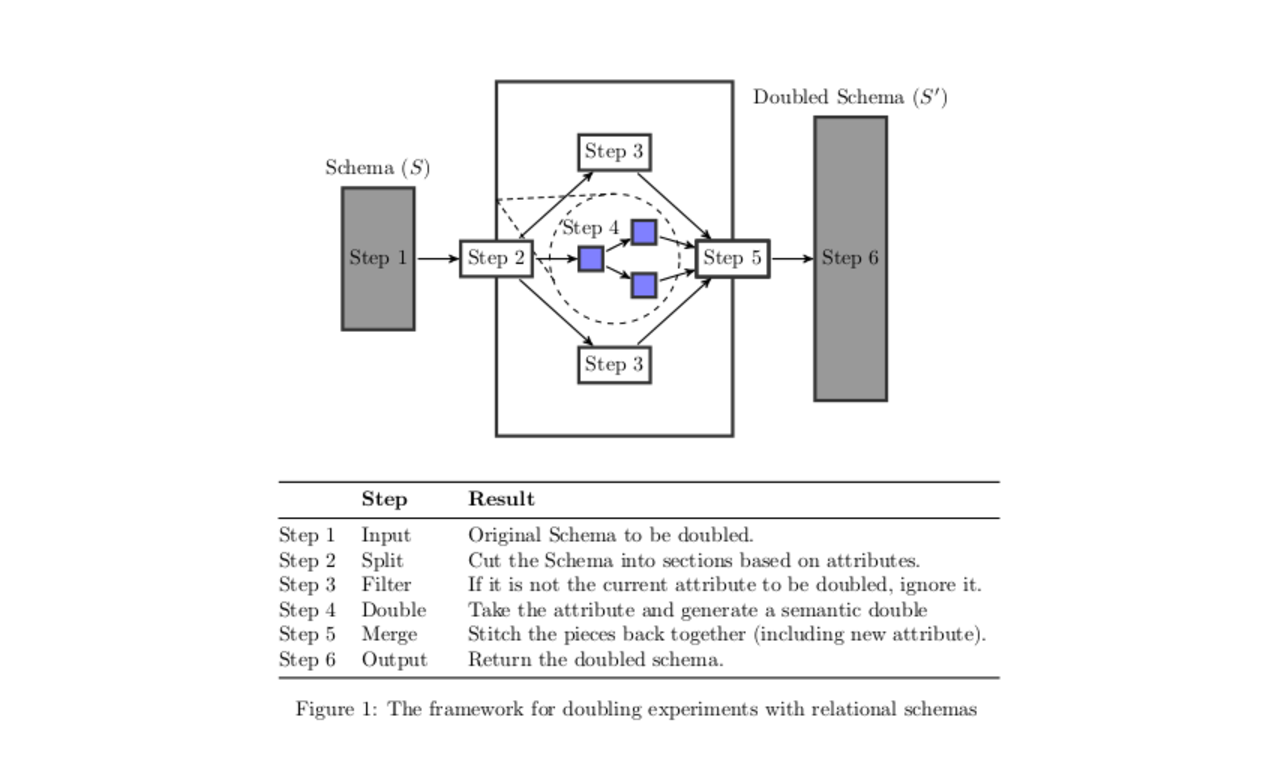
\includegraphics[width=1.25\linewidth]{../diagrams/genDouble}
  %   \caption{Multi Purpose Double Program.}
  %   \label{fig:generaldouble}
  % \end{figure*}

  A relational database schema contains tables, columns, and can contain constraints; 
  all of these items are subject to individual or grouped double. An example of
  both being \textbf{Double Tables}, which doubles all doubles but keep
  everything else constant and also \textbf{Double TablesColumns}, which
  doubles both tables and columns, but keeps everything else the same. That 
  being said, more than one algorithm for doubling is needed, but the same 
  general format is the same for all doubles.

  An example of a general semantic doubling is shown in
  Figure~\ref{fig:generaldouble}.

  \subsection{Automatic Experiment}
  \label{subsec:experiment}

  To determine worst case complexity, an input $n$ is doubled until the 
  ratio $f(2n) / f(n)$ converges to a stable value. To account for random
  error, every time $n$ is doubled, $f(n)$ is recorded ten times, and the
  median time is used for calculating the ratios.  We chose
  median to minimize the effect of outliers. If mean is used instead, a
  single abnormally long run could have a large effect on the result. The overall 
  structure of the experiment is shown in Algorithm~\ref{alg:main}, and in
  Figure~\ref{fig:doublingexp}.

  \begin{figure*}
    \centering
    \centering
    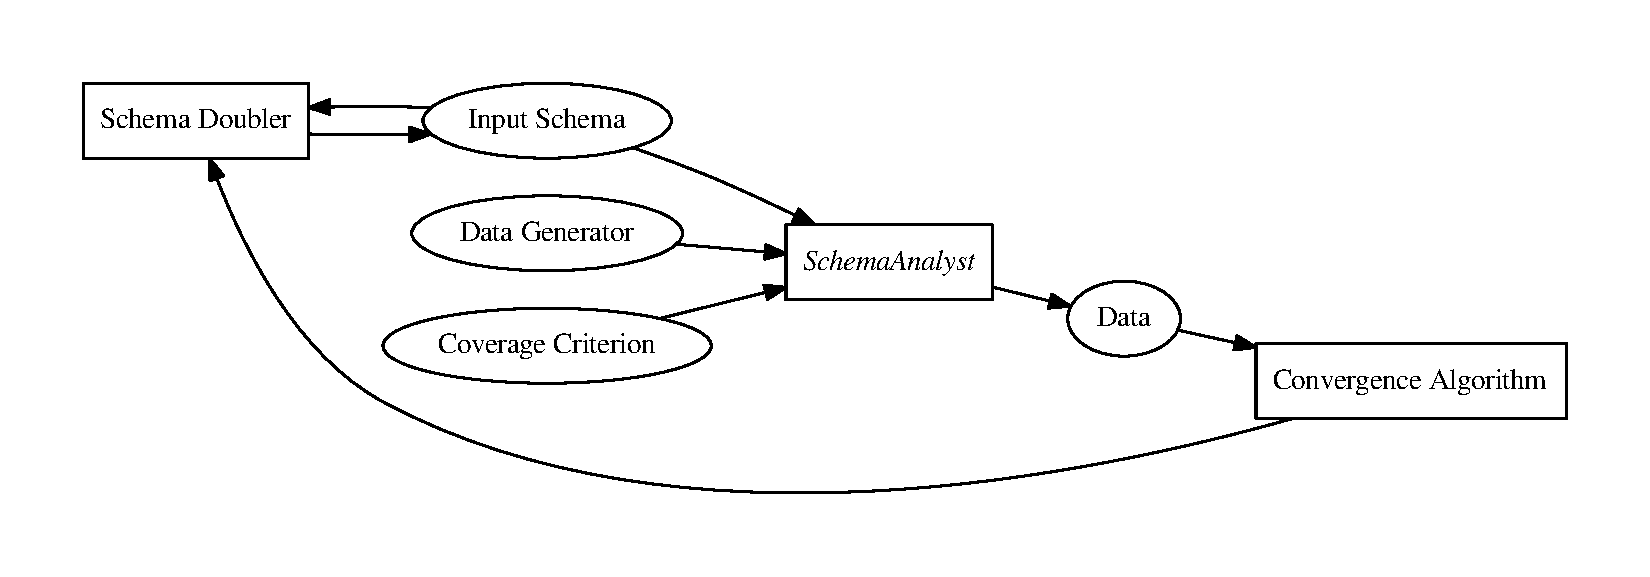
\includegraphics[width=.5\linewidth]{../diagrams/doublingexp.pdf}
    \caption{Technique for conducting automatic doubling experiments.}
    \label{fig:doublingexp}
  \end{figure*}


  This convergence checking is necessary because of the fact that worst-case
  time is only apparent for large values of $n$. If too few doubles
  are tried, then the experiment may terminate before $n$ reaches a value
  where the true worst-case time complexity is apparent. At the same time,
  for inefficient  algorithms, each additional doubling run incurs a substantial
  time overhead. For the sake of efficiently, the experiment should
  terminate as quickly as possible.
  To test for convergence, the last four ratios are compared, and the
  sum of differences between them is compared to a tolerance value. The
  convergence algorithm is shown as Algorithm~\ref{alg:convergence}.

  Another consequence of worst-case time only being apparent for large
  $n$, is that a very small initial $n$ may appear to converge to one,
  which indicates constant time. To prevent the
  experiment from incorrectly terminating given a small starting $n$, we
  require that a program under study display a ratio of one for many
  runs before judging that the ratio does in fact converge to one. Because 
  one signifies constant or logarithmic 
  time, requiring these doubles does not significantly increase the time needed
  to run the experiment, while providing assurance that a small ratio is not due
  to an insufficiently small $n$. This rule is shown in 
  Algorithm~\ref{alg:tuning}.

  \begin{algorithm}[t]
    \caption{Run Doubling Experiment}
    \begin{algorithmic}
      \WHILE{Not Convergent || N not large enough}
      \FOR{$\mathit{trials}$}
      \STATE Run Test
      \ENDFOR
      \STATE Double Schema
      \ENDWHILE
    \end{algorithmic}
    \label{alg:main}
  \end{algorithm}

  \begin{algorithm}[t]
    \caption{Convergent}
    \begin{algorithmic}
      \STATE difference $= |(r_4 - r_3) + (r_3 -r_2) + (r_2 - r_1)|$
      \IF{difference $< \mathit{differanceTolerance}$}
      \RETURN Ratio is convergent
      \ELSE
      \RETURN Ratio is not convergent
      \ENDIF
    \end{algorithmic}
    \label{alg:convergence}
  \end{algorithm}

  \begin{algorithm}[t]
    \caption{N Large Enough}
    \begin{algorithmic}
      \IF{ratio $\approx 1$}
      \IF{number of doubles $< \mathit{doublesTolerance}$}
      \RETURN N is not large enough
      \ENDIF
      \ENDIF
      \RETURN N is large enough
    \end{algorithmic}
    \label{alg:tuning}
  \end{algorithm}

%!TEX root=../seke.tex
% mainfile: ../seke.tex

\begin{table}[t]
  \centering

  \begin{tabular}{r | c c c}
                           Schema  & Tables & Columns & Constraints \\ \hline
    BioSQL                   & 28     & 129     & 186 \\
    Cloc & 2 & 10 & 0 \\
    iTrust & 42 & 309 & 134 \\
    JWhoisServer & 6 & 49 & 50 \\
    NistWeather & 2 & 9 & 13 \\
    NistXTS748 & 1 & 3 & 3 \\
    NistXTS749 & 1 & 3 & 3 \\
    RiskIt & 13 & 57 & 36 \\
    UnixUsage & 8 & 32 & 24 
  \end{tabular}

  \caption{Database schemas used in the experiments.}~\label{tab:schemas}
\end{table}

\vspace{-.05in}
\section{Empirical Analysis}
\vspace{-.05in}

\textbf{Experimental Design}. To gain a full picture of the performance trade-offs, we conducted an experiment for every
configuration of the parameter space (i.e., schema, coverage criterion, data generator, and doubling technique).

In our experimental study, we set $\mathit{tolerance}$ to $0.40$ and $\mathit{lookback}$ to $4$. These values were
chosen by performing doubling experiments on various algorithms, with known worst-case time complexities, and observing
that the ratio converged to the correct value with this configuration.  In an effort to ensure good picks for
parameters, we also conducted preliminary experiments. We set $\mathit{minimum}$ to $20$ after observing that
\textit{SchemaAnalyst} stopped displaying constant behavior after around 5 doubles.  Preliminary studies showed that
while experiments for fast configurations could be completed in less than an hour, slower configurations required days.
Since there are over four thousand possible configurations, the study requires a substantial amount of computational
resources.  As a solution, we conducted the experiments on a high-performance computing (HPC) cluster containing 195
worker nodes of various hardware configurations, ranging from 12 to 16 CPU cores and 24 to 256 GB of memory, and using
the 64-bit Redhat operating system.

% GMK NOTE: It would be better to call this a tree model instead of a regression tree -- the word regression is also
% used in the software testing literature to have a different meanining.

% Regression tree
% Belongs with results_trees, but must be here for page placement within the paper


\section{Results}
  \label{sec:results}

Our experiments reveal that the number of tables in the schema has the
greatest impact on the runtime of \textit{SchemaAnalyst}. The BigOh
complexity\dots 
%TODO need to analyze BigOh

To gain a more nuanced understanding of the results, we construct a
regression tree predicting runtime by the predictors \texttt{Tables,
Columns, Uniques, NotNulls, Checks, Criterion, and DataGenerator}. The
package \textit{ctree} for the R language was used to produce the tree,
shown as Figure~\ref{fig:atree}. The regression tree confirms that the
number of tables has the largest impact on runtime, as can be seen by
the fact that the node 1 splits on the number of tables, and the
significant difference between nodes 6 and 7, which are also
distinguished by the number of tables according to node 5. The tree also
reveals that when the number of tables in the schema is small, the
choice of coverage criterion is the most important predictor for
runtime.  This is shown by node 2, however, the nodes resulting from this
prediction, nodes 3 and 4, do not seem very distinct.  

To gain more insight into the behavior of \textit{SchemaAnalyst} when
the number of tables is small, a new tree was constructed with the same
parameters, with the exception that \texttt{Tables} was removed from
the list of predictors. The resulting regression tree is shown as
Figure~\ref{fig:ttree}.  Node 1 in the new tree also indicates that
the choice of criterion has the largest impact when the number of tables
is not considered.  Node 2 shows that the next most significant
predictor is the data generator, and node 3 shows the next most
significant factor is the number of columns in the schema.  The
differences between the leaves of the tree however, are still not
readily apparent. 

According to the decisions produced by the regression tree, the choice
of coverage criterion and data generator have an impact on the runtime
of \textit{SchemaAnalyst}. To show the effect of these choices, we
present Figure~\ref{fig:crites}, which shows the effect of coverage
criterion on runtime, and Figure~\ref{fig:datas}, which shows the effect
of data generator on runtime.  

For coverage criteria, the most apparent pattern is that AUCC,
ClauseAICC, and CondAICC seem to cause runtime to increase by about the
same amount, with the other criterions taking roughly the same amount of
time.

For data generator, the Random and Random defDults generators took the
most amount of time by a distinctive margin, and a less pronounced
hierarchy between AVM, AVM defaults, Directed Random, and Directed
Random Defaults can be observed.  

While the box and whisker plots allow us to see how choices between
coverage criterions and data generators affects runtime, the question
remains if these differences are statistically and practically
significant. To answer this question, we present the Wilcoxon rank sum
test and the $\hat{A}_{12}$ test.  

%TODO talk about what the tests mean, how to interpret results here

We perform these tests for every pair
of coverage criterions, and every pair of data generators.
Table~\ref{tab:crites} shows the results of these tests for coverage
criteria, and Table~\ref{tab:datas} shows the results for data
generators.

\begin{figure*}
\centering
  \centering
  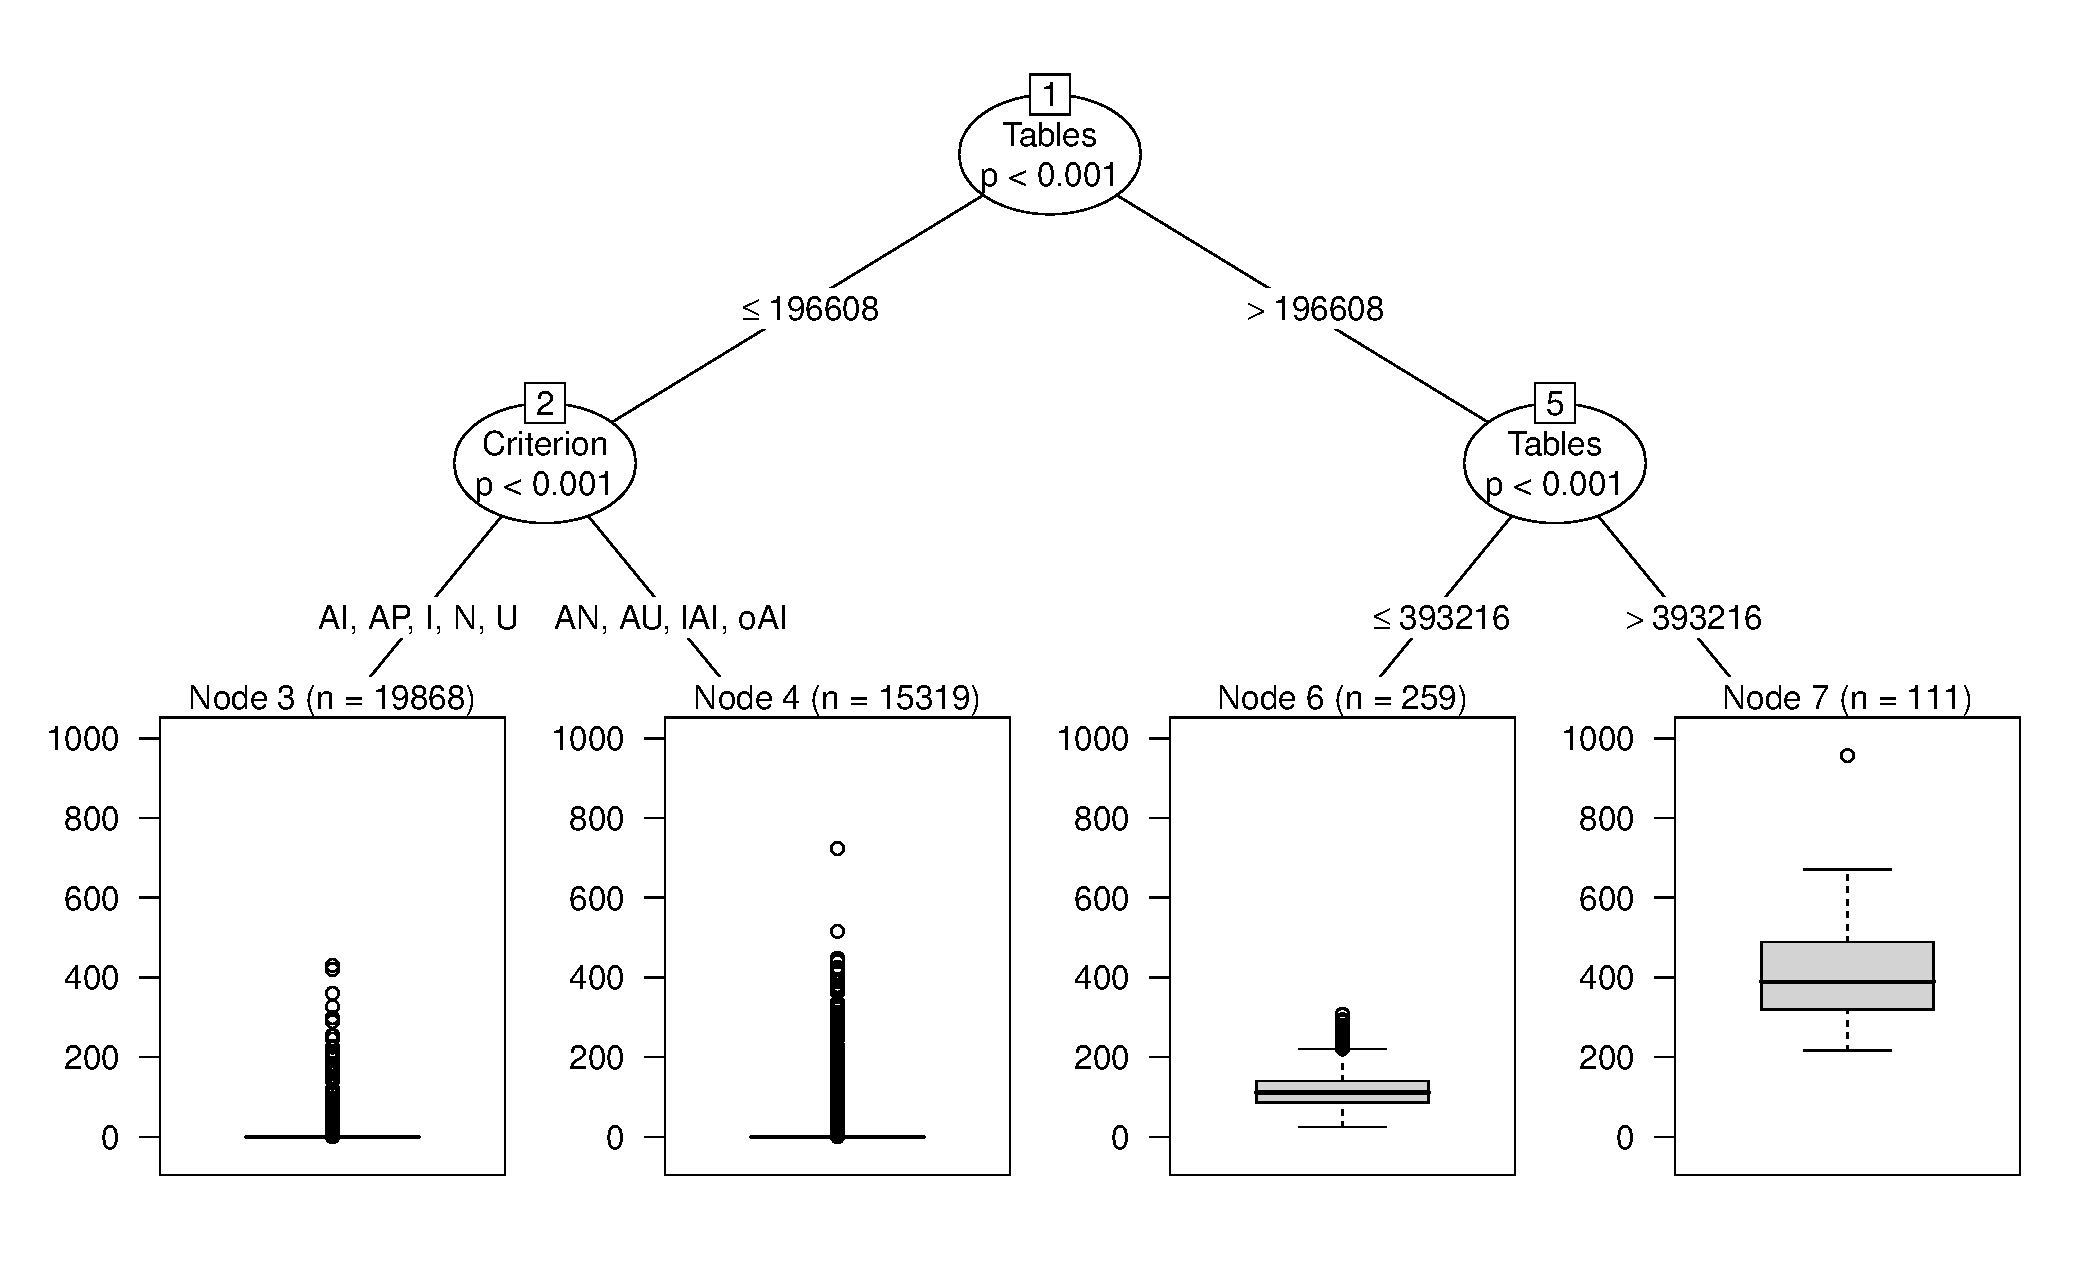
\includegraphics[width=.75\linewidth]{../diagrams/AllTree.pdf}
  \caption{Regression tree using all variables to predict runtime in
  minutes. \vspace{-.15in}}
  \label{fig:atree}
  \vspace{-.15in} 
\end{figure*}

\begin{figure*}
\centering
  \centering
  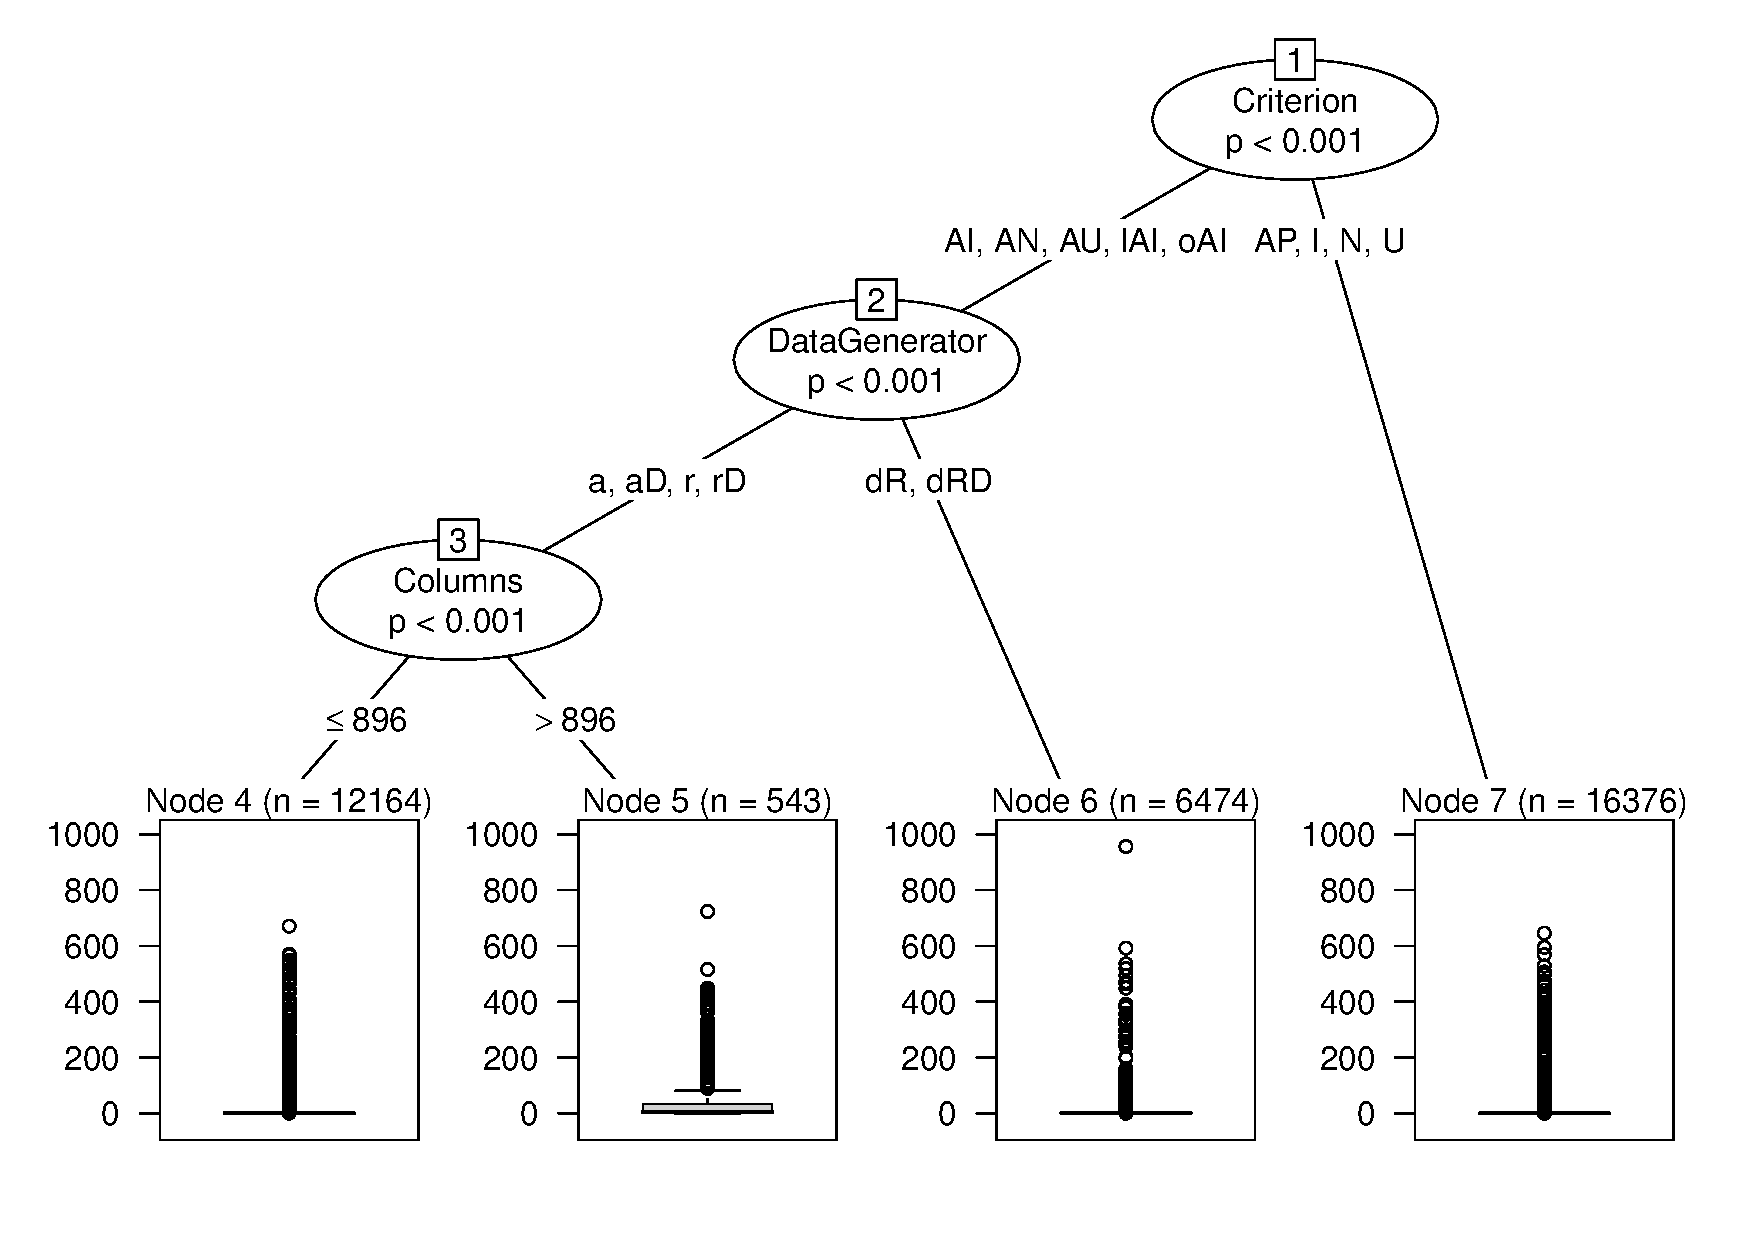
\includegraphics[width=.75\linewidth]{../diagrams/NoTableCtreesd.pdf}
  \caption{Regression tree predicting runtime excluding Tables.\vspace{-.15in}}
  \label{fig:ttree}
  \vspace{-.15in} 
\end{figure*}


\begin{figure}
\centering
  \centering
  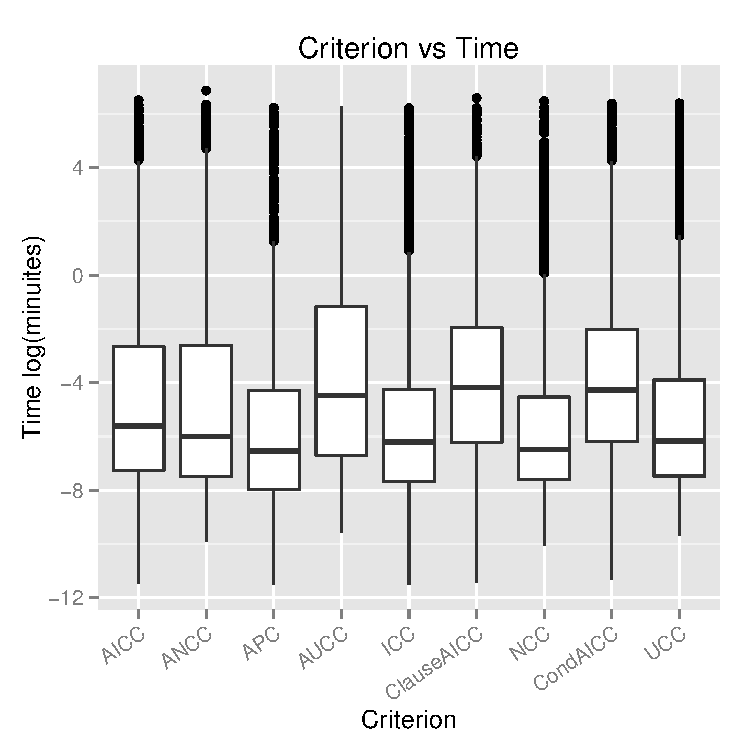
\includegraphics[width=1\linewidth]{../diagrams/CriterionvsTime.pdf}
  \caption{Coverage criterion versus runtime in minutes.\vspace{-.15in}}
  \label{fig:crites}
  \vspace{-.15in} 
\end{figure}

\begin{figure}
\centering
  \centering
  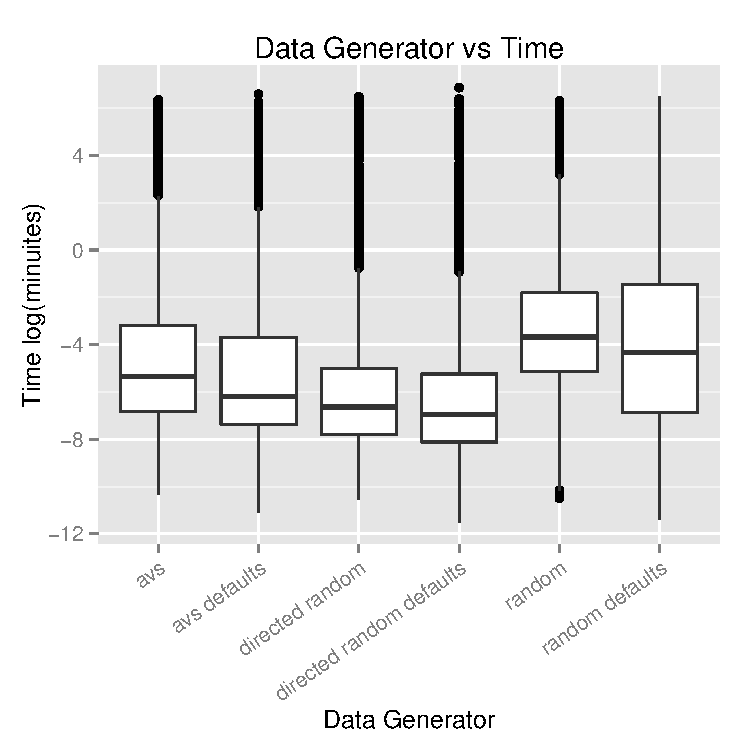
\includegraphics[width=1\linewidth]{../diagrams/DataGeneratorvsTime.pdf}
  \caption{Data generator versus runtime in minutes.\vspace{-.15in}}
  \label{fig:datas}
  \vspace{-.15in} 
\end{figure}


\begin{table*}[h]
\begin{tabular}{llllllllll}
           & APC      & ANCC     & CondAICC & NCC      & AUCC     & AICC     & ClauseAICC & ICC      & UCC   \\ 
APC        & NA       & \cellcolor{gray!25}0.425    &
\cellcolor{gray!45}0.337    & 0.484    &\cellcolor{gray!45} 0.334    &
\cellcolor{gray!25}0.413    &\cellcolor{gray!45} 0.329      & 0.481    & 0.449 \\
ANCC       & 2.20E-16 & NA       &\cellcolor{gray!25} 0.407
&\cellcolor{gray!25} 0.561    &\cellcolor{gray!25} 0.405    & 0.484
&\cellcolor{gray!25} 0.399      & 0.554    & 0.526 \\
CondAICC   & 2.20E-16 & 2.20E-16 & NA       &\cellcolor{gray!45} 0.671
& 0.503    &\cellcolor{gray!25} 0.581    & 0.492
&\cellcolor{gray!45} 0.656    &\cellcolor{gray!25} 0.634 \\
NCC        & 1.20E-02 & 2.20E-16 & 2.20E-16 & NA
&\cellcolor{gray!45} 0.335    &\cellcolor{gray!25} 0.417
&\cellcolor{gray!45} 0.322      & 0.491    & 0.461 \\
AUCC       & 2.20E-16 & 2.20E-16 & \cellcolor{gray!65}6.92E-01 & 2.20E-16 & NA       &
\cellcolor{gray!25}0.577    & 0.490      &\cellcolor{gray!45} 0.651
&\cellcolor{gray!25} 0.628 \\
AICC       & 2.20E-16 & 1.70E-02 & 2.20E-16 & 2.20E-16 & 2.20E-16 & NA
&\cellcolor{gray!25} 0.412      &\cellcolor{gray!25} 0.571    & 0.547 \\
ClauseAICC & 2.20E-16 & 2.20E-16 & \cellcolor{gray!65}2.72E-01 & 2.20E-16 & 1.40E-01 &
2.20E-16 & NA         & \cellcolor{gray!45}0.662    &\cellcolor{gray!45} 0.641 \\
ICC        & 4.00E-03 & 2.20E-16 & 2.20E-16 &\cellcolor{gray!65} 1.83E-01 & 2.20E-16 & 2.20E-16 & 2.20E-16   & NA       & 0.472 \\
UCC        & 9.30E-16 & 3.83E-05 & 2.20E-16 & 7.36E-10 & 2.20E-16 & 5.73E-13 & 2.20E-16   & 9.29E-06 & NA    \\ 
\end{tabular}
\caption{For each pair of coverage criterions, lower left shows Wilcox
Rank Sum Test, upper right shows $\hat{A}_{12}$.}
\label{tab:crites}
\end{table*}


\begin{table*}[h]
\begin{tabular}{lllllll}
                         & Random   & Random Defaults & Directed Random & Directed Random Defaults & AVM      & AVM Defaults \\
Random                   & NA       & 0.538
&\cellcolor{gray!65} 0.740           &\cellcolor{gray!65} 0.789
&\cellcolor{gray!25} 0.627    &\cellcolor{gray!45} 0.680        \\
Random Defaults          & 6.59E-13 & NA              &
\cellcolor{gray!45}0.673           &\cellcolor{gray!45} 0.701
&\cellcolor{gray!25} 0.564    & \cellcolor{gray!25}0.617        \\
Directed Random          & 2.20E-16 & 2.20E-16        & NA
& 0.543                    &\cellcolor{gray!25} 0.360    &\cellcolor{gray!25} 0.435        \\
Directed Random Defaults & 2.20E-16 & 2.20E-16        & 9.74E-16
& NA                       &\cellcolor{gray!45} 0.328    &\cellcolor{gray!25} 0.395        \\
AVM                      & 2.20E-16 & 2.20E-16        & 2.20E-16
& 2.20E-16                 & NA       &\cellcolor{gray!25} 0.572        \\
AVM Defaults             & 2.20E-16 & 2.20E-16        & 2.20E-16        & 2.20E-16                 & 2.20E-16 & NA          
\end{tabular}
\caption{For each pair of Data Generators, lower left shows Wilcox Rank
Sum Test, upper right shows $\hat{A}_{12}$.}
\label{tab:datas}
\end{table*}


\subsection*{Threats to Validity}

Our technique for doubling the number of check constraints on the schema
is simply to duplicate the existing check constraints. It is possible
that \textit{SchemaAnalyst} does less work processing these copied check
constraints than it would given unique check constraints. However,
doubling the check constraints in this way is an easy to implement,
semantically significant way of evaluating \textit{SchemaAnalyst}.

Additionally, since worst-case time is only apparent for large $n$, 
it is possible that the experiment terminated too quickly.  To guard 
against this problem, Algorithms~\ref{alg:convergence} and~\ref{alg:tuning}
were tested on various other algorithms with known worst-case complexities, and 
found to be reliable.

\section{Related Work}

  %TODO GMK: We need more of this
  % Even if you know of some papers, you can send some to me and I can read them

  Goldsmith et al. \cite{Goldsmith:2007:MEC:1287624.1287681} 
  developed a system to empirically evaluate computational
  complexly.  Their system, \textit{Trend-Prof}, uses code
  instrumentation to count the number of times each block 
  of code is executed, and then
  groups these blocks by their behavior.  \textit{Trend-Prof} takes in a
  collection of workloads, user specified features of the workloads, and
  the program to be studied. This technique results in a more powerful
  analysis. However, the authors do not address the
  issue of generating the workloads necessary to achieve a meaningful
  result, and we attempt to do this automatically.  Additionally, our
  approach is novel because we apply it to a domain where the
  theoretical scalability is not yet known.

%!TEX root=../seke.tex
% mainfile: ../seke.tex

\section{Conclusions and Future Work}

% The automated doubling experiment was able to determine the worst case time complexity of \textit{SchemaAnalyst} with
% respect to the number of check constraints in the input schema, for the \textsc{constraintCACCoverage} criterion and the
% \textsc{directedRandom} data generator.  Additional experiments will be conducted on other criteria and data generators.
% Additionally, other factors that may influence the runtime of schema analysis, such as the number of primary keys,
% foreign keys, tables, columns, etc will be investigated.

This paper presented an automated method for empirically suggesting the worst-case time complexity of search-based test
data generation methods. Focusing on the domain of relational database schemas, our approach repeatedly doubles the size
of the input schema and observes the commensurate change in runtime. Although some results are inconclusive, we find
that, in many cases, data generation is linear or linearithmic and, in others, it is quadratic, cubic, or worse.  Our
automated method also revealed that, for all of the test adequacy criteria in the subsumption hierarchy presented by
McMinn et al.~\cite{mcminn2015}, stronger criteria always necessitate more time for test data generation.

Since this paper's technique did not consider the doubling of constraints like {\tt FOREIGN KEY}s, future work will
focus on creating doublers for these unstudied constraints. Additionally, the current doubling mechanism avoids
introducing semantically invalid constraints by restating existing constraints; in future work we plan to implement and
evaluate more realistic ways to double relational schemas. Because certain experiments timed out before converging, we
also want to re-run these configurations with longer time limits and more memory. Finally, we will investigate how
automated parameter tuning can support choosing the convergence condition without manual tuning before experimentation
in a new computational environment. Ultimately, the combination of the presented framework with the completed future
work will yield an effective way to empirically understand the worst-case case time complexity of search-based test data
generation for relational database schemas.


{\small 
\bibliographystyle{IEEEtran}
\bibliography{bibtex/seke}
}

\end{document}
